\documentclass{standalone}
\usepackage{tikz}
\usepackage{pgfplots}
\pgfplotsset{width=32cm,height=18cm,compat=1.3}
\pgfplotsset{every tick label/.append style={font=\Huge}}
\usepackage{filecontents}

\usetikzlibrary{patterns}

\definecolor{citrine}{rgb}{0.89, 0.82, 0.04}

\begin{document}
	\centering
		\vspace{1.5em}
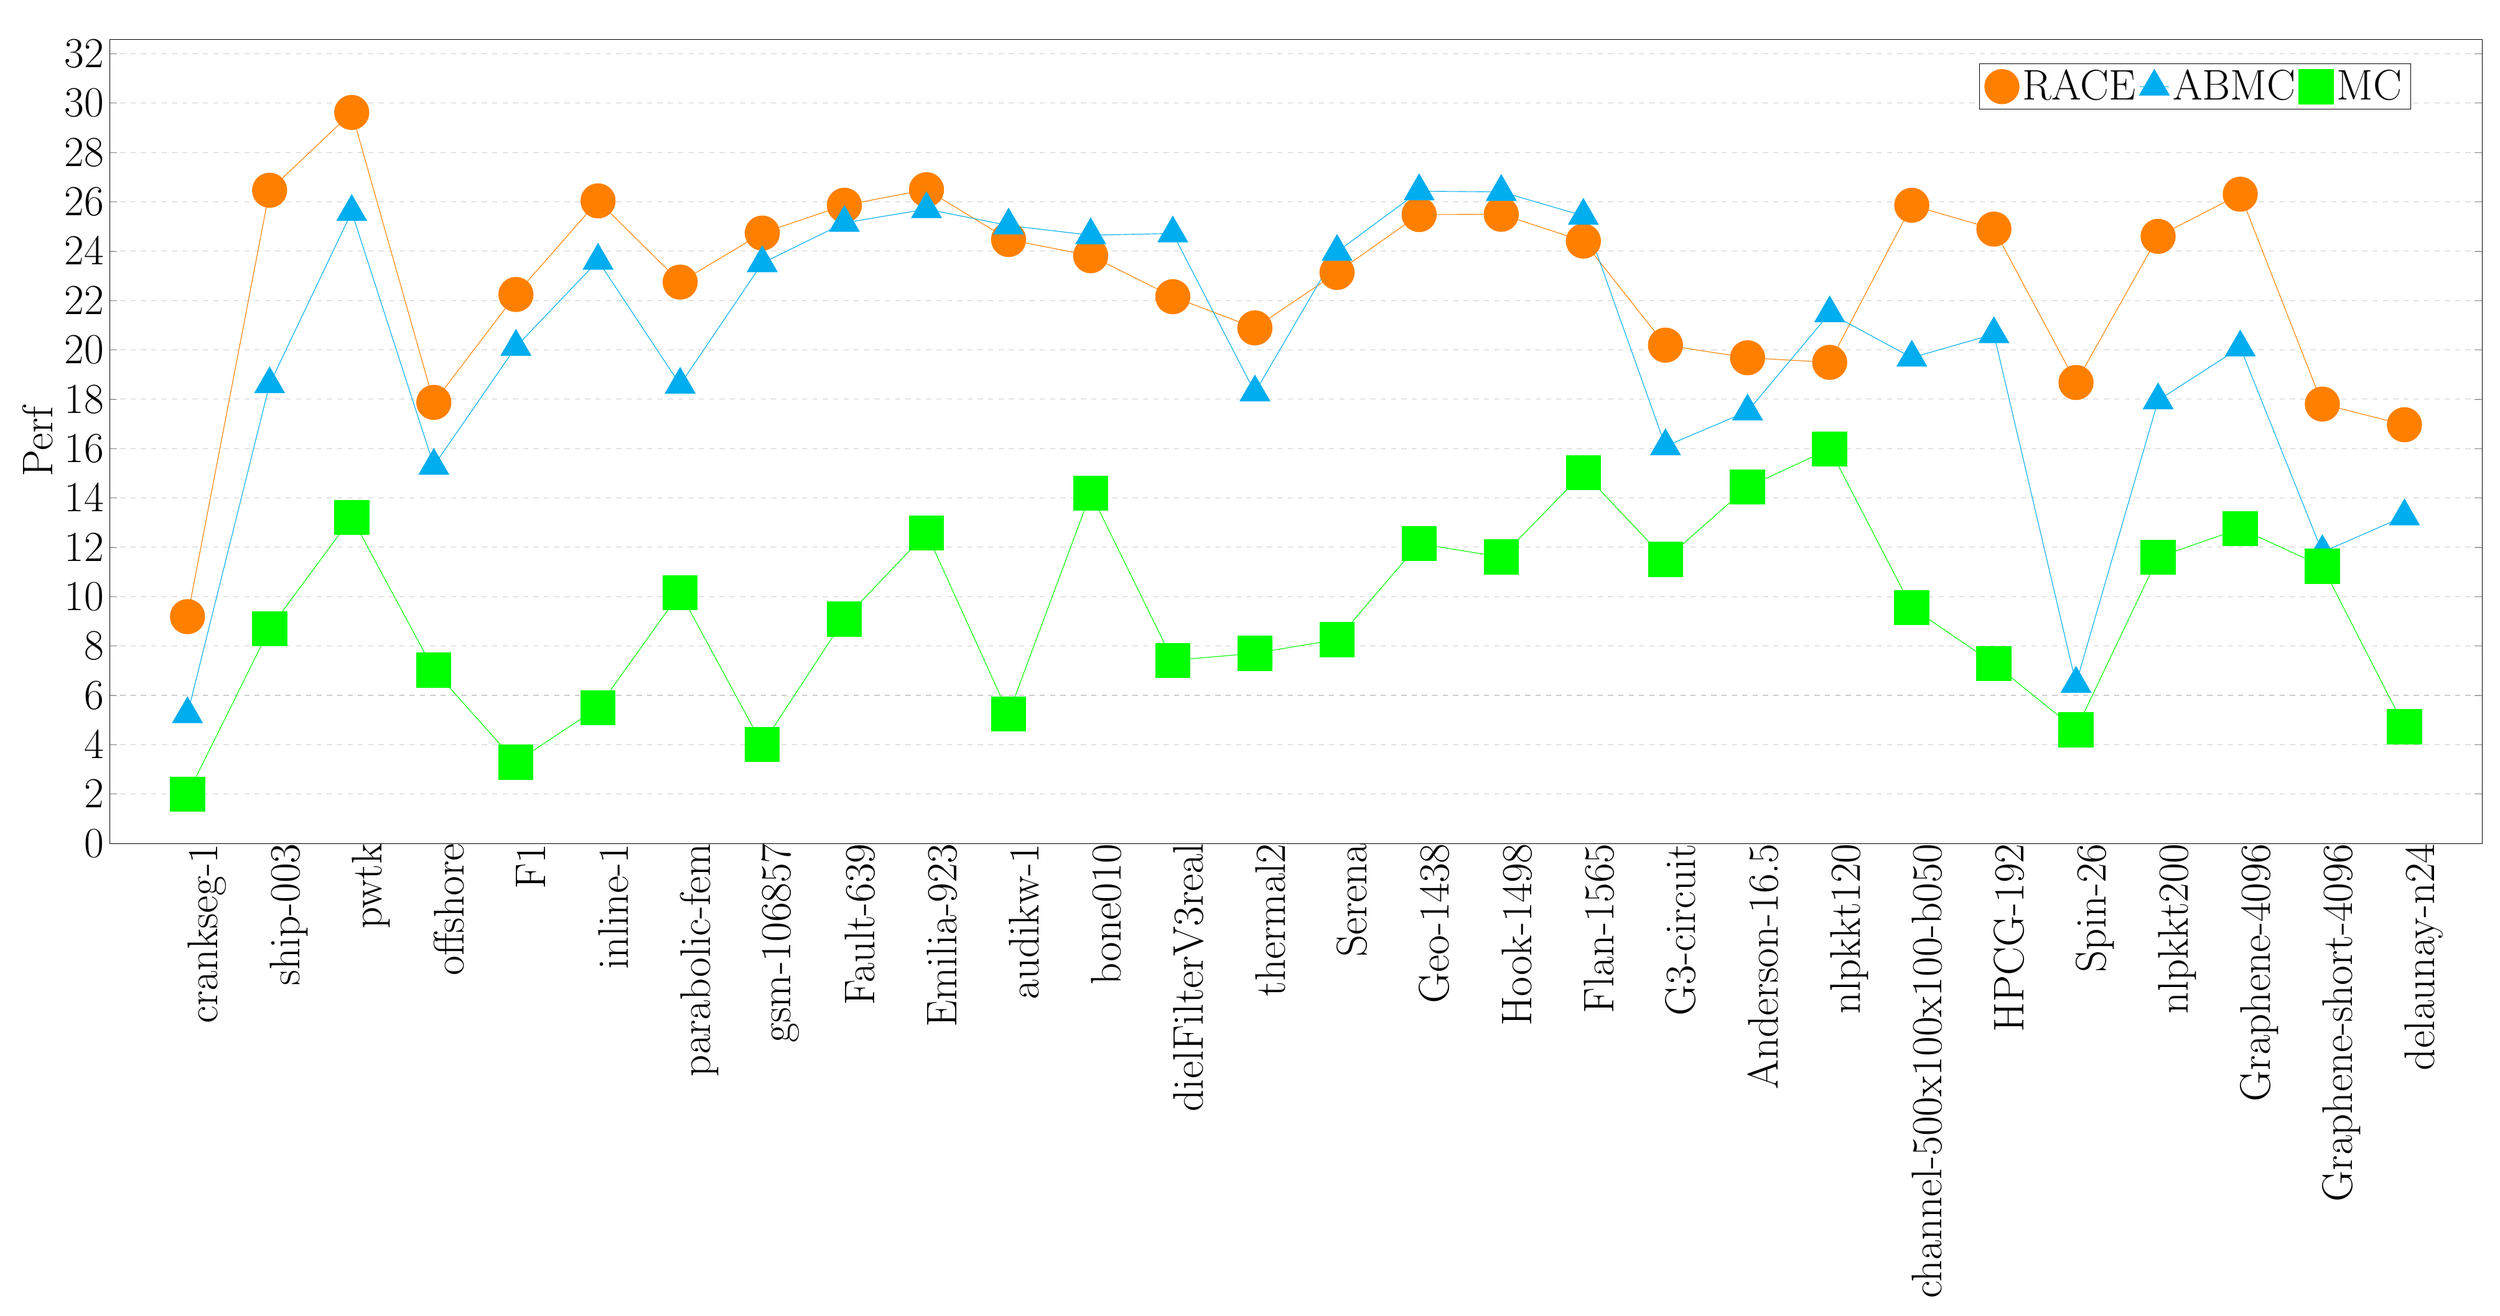
\begin{tikzpicture}
		%	\node at (13.25,15) {\LARGE{}};
			\begin{axis}[
		%	xmin=0.25, xmax=7.25,
			ymin=0, %ymax=3.25,
			xtick={1, 2, 3, 4, 5, 6, 7, 8, 9, 10, 11, 12, 13, 14, 15, 16, 17, 18, 19, 20, 21, 22, 23, 24, 25, 26, 27, 28},
		%	ytick={0,0.5,1,1.5,2,2.5,3},
			xticklabels={crankseg-1, ship-003, pwtk, offshore, F1, inline-1, parabolic-fem, gsm-106857, Fault-639, Emilia-923, audikw-1, bone010, dielFilterV3real, thermal2, Serena, Geo-1438, Hook-1498, Flan-1565, G3-circuit, Anderson-16.5, nlpkkt120, channel-500x100x100-b050, HPCG-192, Spin-26, nlpkkt200, Graphene-4096, Graphene-short-4096, delaunay-n24},
			width  = 50cm,
			height = 18cm,
			major x tick style = transparent,
			%	minor ytick={1, 5, 10, 15, 20, 25, 30 ,35,40},
			grid = minor,	
			%add_bar_commands
			ymajorgrids = true,
			grid style={dashed, gray!40},
			ylabel = {\Huge{Perf}},
		%	symbolic x coords={Graphene-2048-2048, Graphene-4096-4096, Spin-24-24-24},
			x tick label style={rotate=90, anchor=north east, inner sep=0mm, font={\Huge}},
			tick label style={font={\Huge}},
			scaled y ticks = false,
			enlarge x limits=0.035,
			legend cell align=left,
			legend style={font=\Huge},
			legend columns=-1,
			legend style={
				%at={(1,1.05)},
				%anchor=south east,
				%column sep=1ex,
				legend pos=north east
			},
			%spl_legend_code
			title= {\Huge\scalebox{1.5}{{}}}
			]

\addplot[mark=*, mark size=10pt, mark options={orange}, draw=orange ] plot coordinates{(1,9.188028) (2,26.465952) (3,29.619693) (4,17.869342) (5,22.243093) (6,26.036429) (7,22.744309) (8,24.731023) (9,25.859193) (10,26.490050) (11,24.470638) (12,23.813569) (13,22.152597) (14,20.888076) (15,23.134373) (16,25.481092) (17,25.492494) (18,24.406704) (19,20.189379) (20,19.678338) (21,19.492790) (22,25.858192) (23,24.893000) (24,18.676146) (25,24.598421) (26,26.306260) (27,17.802001) (28,16.964026)};
\addplot[mark=triangle*, mark size=10pt, mark options={cyan}, draw=cyan ] plot coordinates{(1,5.237748) (2,18.606680) (3,25.587634) (4,15.303070) (5,20.122238) (6,23.611138) (7,18.587763) (8,23.512788) (9,25.145408) (10,25.701974) (11,25.039542) (12,24.643671) (13,24.716414) (14,18.272815) (15,23.969977) (16,26.428093) (17,26.400655) (18,25.433920) (19,16.095095) (20,17.504669) (21,21.481489) (22,19.682763) (23,20.636315) (24,6.466911) (25,17.954247) (26,20.095991) (27,11.802042) (28,13.253567)};
\addplot[mark=square*, mark size=10pt, mark options={green}, draw=green ] plot coordinates{(1,1.991533) (2,8.698461) (3,13.208866) (4,7.025583) (5,3.295957) (6,5.502482) (7,10.155564) (8,4.007839) (9,9.090876) (10,12.578046) (11,5.250340) (12,14.188078) (13,7.415697) (14,7.705833) (15,8.258869) (16,12.147435) (17,11.603119) (18,15.026665) (19,11.507194) (20,14.443050) (21,15.984644) (22,9.552907) (23,7.284023) (24,4.604878) (25,11.597878) (26,12.757724) (27,11.231440) (28,4.731314)};
	%addplot cmd

	\legend{RACE, ABMC, MC}

	\end{axis}			
\end{tikzpicture}

\end{document}

